\documentclass{sigchi}

% Remove or comment out these two lines for final version
\toappearbox{\Large Submitted to CHI'13. \\Do not cite, do not circulate.}
\pagenumbering{arabic}% Arabic page numbers for submission. 

% Use \toappear{...} to override the default ACM copyright statement (e.g. for preprints).

% Load basic packages
\usepackage{balance}  % to better equalize the last page
\usepackage{graphicx} % for EPS, load graphicx instead
\usepackage{times}    % comment if you want LaTeX's default font
\usepackage{url}      % llt: nicely formatted URLs
\usepackage{tabularx}
\usepackage{subfigure}

% llt: Define a global style for URLs, rather that the default one
\makeatletter
\def\url@leostyle{%
  \@ifundefined{selectfont}{\def\UrlFont{\sf}}{\def\UrlFont{\small\bf\ttfamily}}}
\makeatother
\urlstyle{leo}


% To make various LaTeX processors do the right thing with page size.
\def\pprw{8.5in}
\def\pprh{11in}
\special{papersize=\pprw,\pprh}
\setlength{\paperwidth}{\pprw}
\setlength{\paperheight}{\pprh}
\setlength{\pdfpagewidth}{\pprw}
\setlength{\pdfpageheight}{\pprh}

% Make sure hyperref comes last of your loaded packages, 
% to give it a fighting chance of not being over-written, 
% since its job is to redefine many LaTeX commands.
\usepackage[pdftex]{hyperref}
\hypersetup{
pdftitle={SIGCHI Conference Proceedings Format},
pdfauthor={LaTeX},
pdfkeywords={SIGCHI, proceedings, archival format},
bookmarksnumbered,
pdfstartview={FitH},
colorlinks,
citecolor=black,
filecolor=black,
linkcolor=black,
urlcolor=black,
breaklinks=true,
}

% create a shortcut to typeset table headings
\newcommand\tabhead[1]{\small\textbf{#1}}


% End of preamble. Here it comes the document.
\begin{document}

\title{Touch keyboard hierarchical spatial models with back-offs for personal 
and hand posture adaptation}

% Note that submissions are blind, so author information should be omitted
\numberofauthors{3}
\author{
  \alignauthor 1st Author Name\\
    \affaddr{Affiliation}\\
    \affaddr{Address}\\
    \email{e-mail address}\\
  \alignauthor 2nd Author Name\\
    \affaddr{Affiliation}\\
    \affaddr{Address}\\
    \email{e-mail address}\\
  \alignauthor 3rd Author Name\\
    \affaddr{Affiliation}\\
    \affaddr{Address}\\
    \email{e-mail address}\\
}

% Teaser figure can go here
%\teaser{
%  \centering
%  \includegraphics{Figure1}
%  \caption{Teaser Image}
%  \label{fig:teaser}
%}

\maketitle

\begin{abstract}
In this sample paper, Sheridan Printing Co., Inc. 
describe the formatting requirements for
SIGCHI Conference Proceedings, and this sample file
offers recommendations on writing for the worldwide
SIGCHI readership. Please review this document even if
you have submitted to SIGCHI conferences before, some
format details have changed relative to previous years.
\end{abstract}

\keywords{
	Guides; instructions; author's kit; conference publications;
	keywords should be separated by a semi-colon.
	\\\textcolor{red}{Mandatory section to be included in your final version.}
}

\category{H.5.m.}{Information Interfaces and Presentation (e.g. HCI)}{Miscellaneous
\\
\textcolor{red}{See: \url{http://www.acm.org/about/class/1998/}
for more information and the full list of ACM classifiers and descriptors. 
Mandatory section: On the submission page
only the classifiers' letter-number combination will need to be entered.}
}

\terms{
	Human Factors; Design; Measurement. 
	If you choose more than one ACM General Term, 
	separate the terms with a semi-colon.
\\
\textcolor{red}{If you choose more than one ACM General Term, 
separate the terms with a semi-colon. See list of ACM terms at:
\url{http://www.sheridanprinting.com/sigchi/generalterms.htm}.
Optional section to be included in your final version.}
}

\section{Introduction}
Modern touch screen keyboards are error-tolerant. They can correct sloppy touch
events to user intended words based on a combination of language model predictions and a spatial model estimation. 
The spatial model that converts a touch point into the probabilities of keys 
depends on a number factors: hand-posture (e.g. two thumbs vs. one finger input \cite{Azenkot:2012}), 
the individual \cite{Findlater:2012} and the target key's position \cite{Azenkot:2012}.

In this paper we explore different ways of touchscreen keyboard adaptation and
their effects in key detection accuracy and auto-correction with language
models. The adataptions we consider are key, posture and individual adaptations. By key adaptation,
we mean each key has its own spatial model instead of sharing the same model. For instance, 
the simplest key detection method which finds the closest key to the touch point is not key adpative,
because it assumes each key has the same offset from the center of the bounding box 
of the key and same covariance matrix if
we model the touch point distribution as a bi-variate Gaussian distribution.  

The paper makes the following contributions. First
We propose a hierarchical adaptive spatial model that combines different
ways of spatial adaptation to improve the key detection accuracy, and provides seamless back-offs when necessary.

 1. Spatial model building
2. Hand-posture classifier
3. User adaptation
4. Key detection process

\section{Related Work}
There is a body of active research on combining spatial model and language model
to improve text entry accuracy on a soft touch screen keyboard. As our focus is on the 
sptial model, we will also mainly look at the related work in spatial model.    

In terms of key adaptation (i.e. each key has its own model instead of
sharing the same model), Goodman et al. \cite{Goodman:2002} use bi-variate Gaussian distribution with means, and
covariance matrices computed separately for each key.


Gunawardana et al. 
The prior work from Findlater et al. [2] suggests that personalized touch 
keyboard which adapts its underlying key-press classification models to the 
users can improve typing speed.  But they assume that the same individual would 
maintain the same hand posture. 

We observe that the same individual may change hand posture even on the same device. The study from Azenkot and Zhai [1] shows that there are significant differences in typing speed and error rate between two-thumb input posture and one-finger input posture. More importantly, the horizontal and vertical offsets are different for each key and posture combinations. This suggests that automatic posture detection and posture adaptive spatial model can potentially improve key detection accuracy.

When the user switches hand posture, the adapted spatial model may in fact give less accurate estimations in the transient period of adaptation. To mitigate this problem and consider all the different facets of adaptation, we designed a hierarchical spatial models with back-offs for touch keyboards.  

Our approach consists the following components:

\section{Hierarchical Adaptive Spatial Models}

To incorporate different strategies of adaptations, we propose a hierarchical
spatial model consisting of a number of sub-models.
The entire model can be viewed as a hierarchy of sub-models in different
“orders” (Figure. \ref{fig:hierarchy}).

\begin{figure}[tb]
  \centering
  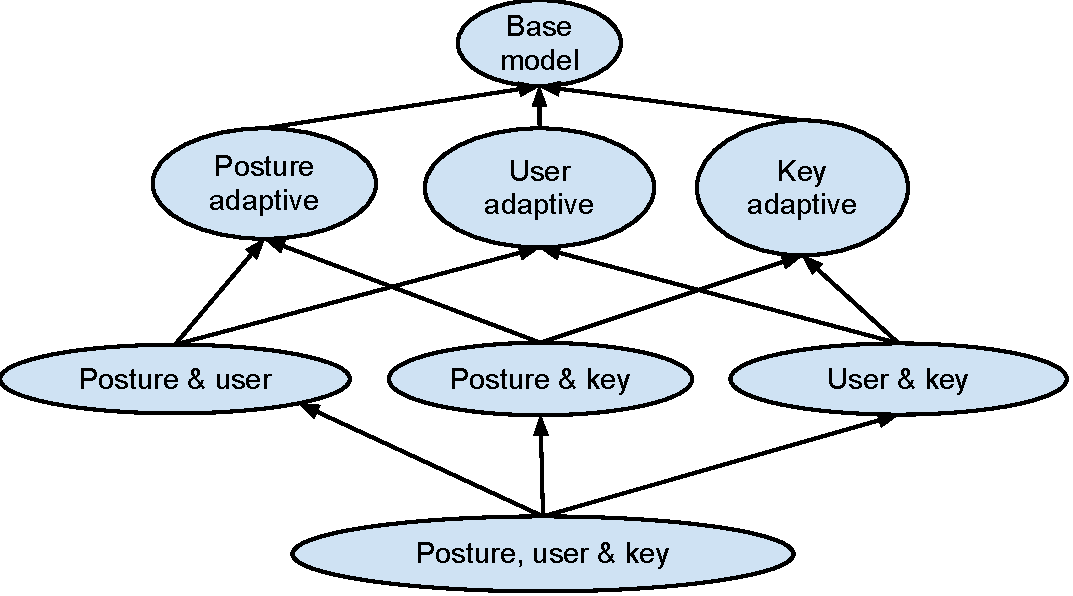
\includegraphics[width=1\columnwidth]{figures/hierarchical-spatial-model.pdf}
  \caption{Hierarchical spatial models}
  \label{fig:hierarchy}
\end{figure}

The zeroth order is the base model which is key, person, and posture
independent. This is the most general model combining all data together. The
higher order models consist of a combination of spatial models that adapt to hand 
posture (e.g. one finger, two thumbs, or ten fingers on tablets) , key or 
bi-letters (e.g. "h/t” where the current target letter is the “h” key and the 
previous letter is “t”), and the individual user. 

The higher the order of the sub-model, the more data is required to build the model because
the model is more complex with more parameters. This means that each combination of the 
conditions needs sufficient number of samples to build a reliable model. Each 
such sub-model would only become active when its reliability passes a set 
threshold (e.g. more than 100 points had been collected); otherwise these models
 that are still “growing” but in “dormant” mode.

\section{Comparison of Spatial Models}
We compare key detection error rate with different models to analyze their
relative effectiveness (Table \ref{tab:comparison}). This can inform us the order of the
back-off models to use when there is not enough data for higher order models.
10-fold cross validation is used, and the training and testing data sets have
different sets of users.

\begin{table} [tb]
  \centering
  \begin{tabular}{|l|c|}
    \hline
    \tabhead{Spatial model} &
    \multicolumn{1}{|p{0.2\columnwidth}|}{\centering\tabhead{Key detection
    error rate}} \\
    \hline
    Distance from the center of the keys & 7.976\% \\
    \hline
    \multicolumn{1}{|p{0.7\columnwidth}|}{Base model (same Gaussian model for
    all the keys with a full covariance matrix)} & 7.853\% \\
    \hline
    Key adaptive model  & 8.023\% \\
    \hline
    Posture and key adaptive model & 7.058\% \\
    \hline
    User and key adaptive model  & 6.845\% \\
    \hline
  \end{tabular}
  \caption{Comparison of key detection accuracy (no language model) with
  different spatial models using 10-fold cross validation.}
  \label{tab:comparison}
\end{table}

Evaluation is based on a data set collected from an earlier study of 32
participants. Users were given target phrases to type on a Nexus S phone. The
details of the study can be found in this paper \cite{Azenkot:2012}. Users were asked to
enter specific phrases. 
We remove the data from 2 left-handed users in our analysis, and are left with
data from 9 users with one index finger input, 11 users with one thumb input and
10 users with two thumbs input.  In our analysis, we combine the data from index finger input
and one-thumb input togetehr. So two postures are considered here: one finger versus two thumbs. We also filtered out points that are 1.5 times
the height of the key away from the center of the target key.

The simpliest base model can have a Gaussian distribution with 0 x and y
mean offsets and the same spherical covariance matrix for all the keys. Key
detection based on this model is essentially choosing the key that has the shortest Euclidean distance from the tapping coordinates. 
One step beyond this is to have a full covriance matrix trained from the
training data, but still using the same Gaussian model for each key.

\subsection{Key Adaptation}
A basic key adaptive model is building a bivariate Gaussian model for each key 
using data from many different users. Then the key detection process involves 
choosing the key whose Gaussian model gives the highest probability for the 
given (x, y) tapping coordinates. When this is combined with posture and 
individual adaptation, more specialized Gaussian models are built for each key.

The difference in key detection accuracy between using the base model only and
the key adaptive model is not big. It is even surprising that key adaptive model
gives slightly lower accuracy. A closer look at the data shows that the most number of error occurs between
``E'' and ``W''. Because there are more one-finger input users in the data set, the 
Gaussian models built for ``E'' and ``W'' have right horizontal offsets. However, for the two thumb input, 
there is usually a left horizontal offsets. Hence there are more errors for tow-thumb input.

This suggests that key adpative model may not be always effectivce unless we have enough data and a balanced
number of postures in the training data. But since the key adaptive model can be trained offline by collecting data from a 
large number of users, this shows that it can be used as the basic backup model once we collect enough data. 

\subsection{Posture Adaptation}
Key adaptation becomes more effective when combined with posture adaptation. There can be different levels of
complexy for posture adapation. For the most complex one, we can build two models for each key for the 
two input posture; or we can do posture adaptation for a certain number of keys. The best result is obtained when we only do 
posture adaptation for the keys on the left side. The error rate for postur and key adaption shown in the table is 
based on posture adaptation for the keys on the left side. Note the choice of this set of keys
is not arbitrary. As observed by Azenkot et al. \cite{Azenkot:2012}, the difference in horizontal
offsets of the touch points from different postures are most prominent for the keys on the
left set (Note that for left-handed users, the reverse is probably true). 
In addition, the analysis of variance based on the tapping coordinates in the data set shows
that, for different postures, there are significant differences in the means of
the $x$ coordinate for the keys on the left side of the keyboard and the
``space'' key ($p < 0.05$). 

There is 12.03\% reduction in error rate compared to key adaptation only. Two
sample one sided paired t-test shows that the improvement in accuracy is
significant when we use posture and key adaptation versus key adaptation only (t = -2.4421, df = 29, p = 0.01047).

Figure \ref{fig:key-boundary} shows the comparison of effective areas of the keys
with different spatial models. Each colored area presents the region such that if the
user tap in that region, the underlying spatial model will classify that key with the 
corresponding key label. Note how the key areas for the left-side keys shift to the left
for two-thumb input and shift slightly to the right for one-finger input.

\begin{figure}[tb]
	\centering
	\subfigure[Key adaptive model]{
    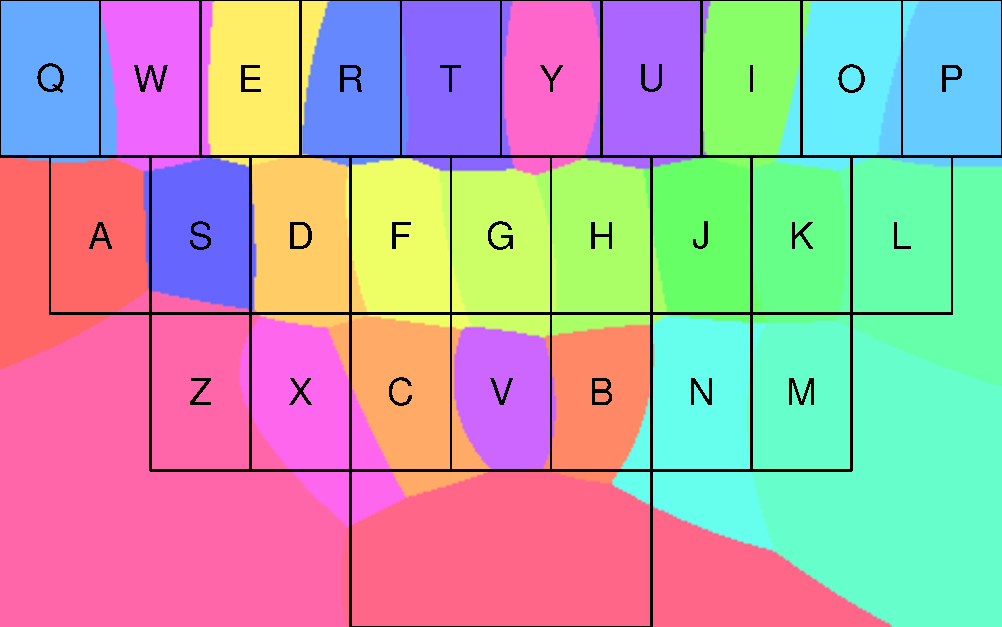
\includegraphics[width=0.47\columnwidth]{figures/key-model.pdf}
    \label{fig:subfig1}
	} ~
	\subfigure[Posture and key adaptive model for one-finger input]{
    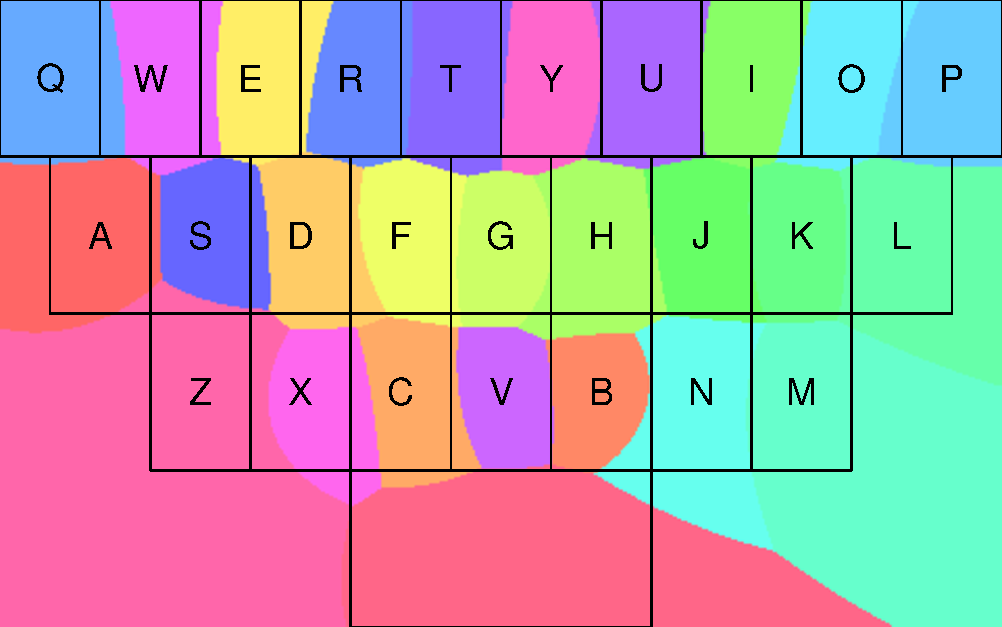
\includegraphics[width=0.47\columnwidth]{figures/posture-t.pdf}
    \label{fig:subfig2}
	}
	\subfigure[Posture and key adaptive model for two-thumb input]{
    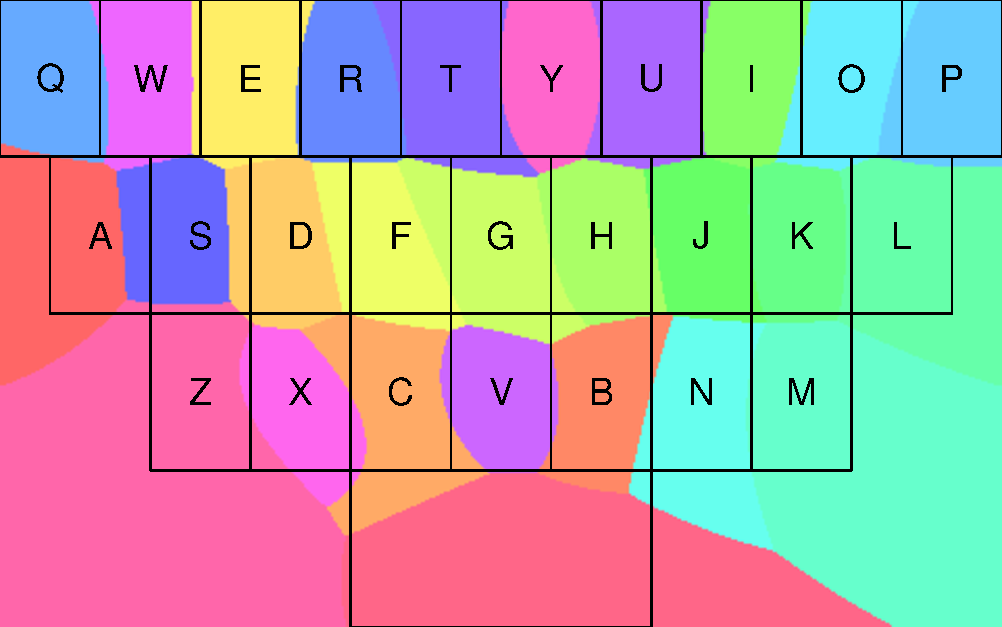
\includegraphics[width=0.47\columnwidth]{figures/posture-tt.pdf}
    \label{fig:subfig3}
	}
	\caption{Comparison of effective key areas with different spatial models}
	\label{fig:key-boundary}
\end{figure}

The accuracy is based on perfect knowledge of the posture which represents an
upper bound for posture adaptation for these data sets. In the actual 
implementation, the posture model can be turned on when we have high enough 
confidence about the posture classification.

\subsection{User Adaptation}
The user and key adaptive model gives the lowest error rate compared to other models. 
This suggests that user and key adaptation can have higher priority in the hierarchy and during
backoff. However, it should also be noted that we need enough data points to build an
accurate model for each key for each individual.
Only when we do not have enough data for the user, we can use posture and key adaptation.

For user and key adaptation, for each fold, we use 90\% of the users to train the
combined back-off key models. Then for each of the 10\% testing users,  a
fraction k of the data for each key is used to train the user adaptive key
models. The accuracy of these data points are tested on the combined key models.
The remaining 50\% of the data for each user are tested on the user adaptive 
models together with the combined model for backup. The backup is used when 
there is not enough data for certain key (we used 10 data points) to build the 
Gaussian model. In this analysis, $k$ is set to be 50\%.

\begin{figure}[tb]
  \centering
  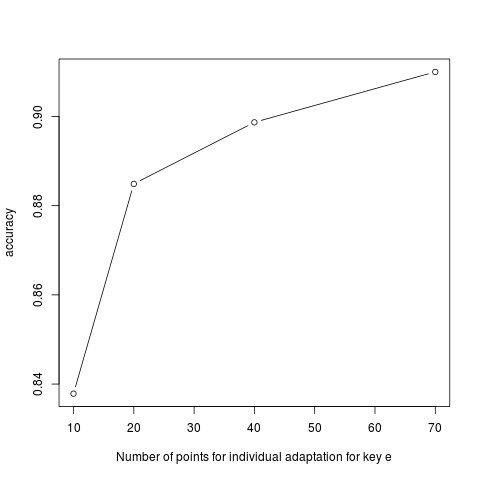
\includegraphics[width=1\columnwidth]{figures/user-adapt-e.png}
  \caption{Tapping points data from input on a Nexus S phone.}
  \label{fig:time-distance}
\end{figure}

The key spatial model can also be more specialized to include bi-letter patterns
that occur frequently, for instances, h followed by e, t followed by h etc. 
Figure 2 shows the (x, y) coordinates of the tapping points for letter “e” from 
one of our data sets, and the 0.95 confidence ellipses of the Gaussian models 
for different conditions. The plot shows that when we combine data for all the 
posture together, the distribution of points for “e” after “h” is very slightly 
different from that of all “e”. But if we look at “e” after “h” for one-finger input (cyan color), the difference is bigger. Another point to note is that, since these are highly frequent patterns, even a small improvement in detecting these keys based on these more specialized models may give a bigger improvement in the overall key detection accuracy.


Figure 2. Comparison of Gaussian models (0.95 confidence ellipses) for letter “e”

\section{Input hand posture adaptation}
To incorporate posture adaptive spatial models, we need to develop a method to
detect users' posture when they are typing on the touch screens. 

\subsection{Hand posture classifier}

We developed a hand-posture classifier that constantly returns an estimate of the user's current posture (two thumbs vs. one finger input).

Our method of hand-posture classification is based on Fitts’ law which states that the time (T) required to move to a target is a function of the distance (D) to the target and the size (W) of the target (Equation 1).
\begin{align}
T = a + b\log_2(1 + \frac{D}{W})
\end{align}                                                  
The insight here is that we expect the one-finger input posture follows this law,  but two-thumbs input may not. For example, when the user types “al”, it takes longer time to type using one finger because the distance between these two keys are large, but with two thumb, it can be very fast because she can use the left thumb to type “a” and the right thumb for “l”.

\begin{figure}[tb]
  \centering
  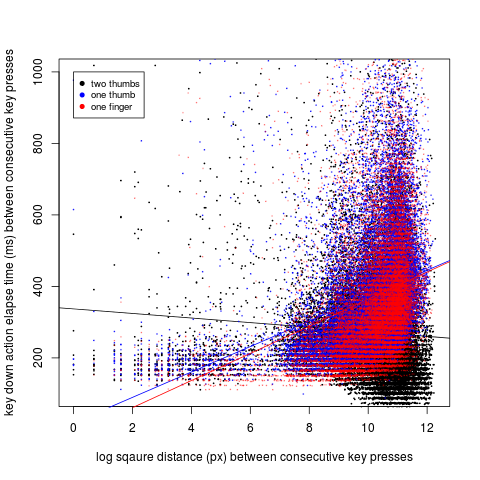
\includegraphics[width=1\columnwidth]{figures/time-distance.png}
  \caption{Tapping points data from input on a Nexus S phone.}
  \label{fig:time-distance}
\end{figure}

Figure. \ref{fig:time-distance} shows the relationship between the time elapsed 
and the log square distance travelled between consecutive key presses. We can
see that for the one-finger input (blue and red points), the time taken
increases with distance whereas for the two-thumb input, there is no obvious
trend. The difference is more significant when the log square distance (natural
log) is greater than 10 px.

Based on this finding, we include the time elapsed and the log square distance
between two consecutive key presses as the features for the posture classifier. 
To account for individual typing speed differences, we also use normalized time 
elapsed between consecutive key presses as the third feature. It is calculated according the following equation:

\begin{align}
\text{Normalized time elapsed} = \frac{\text{time elapsed}}{\text{average time
elapsed for the last 10 key presses}}
\end{align}

We train a SVM classifier with these 3 features for consecutive tap points that 
are on different sides of the keyboard and whose log square distance is at least
10px. We use 70\% of the data for training and 30\% of the
data for testing. The users in the training and testing data sets are different.

The Pepper (84292 filtered data points) data sets we use consist tapping points 
from different users with different postures. The classification accuracy from
the single tap classifier for keys with previous key on the different sides of
the keyboard 83.559\% (11090/13272).

The single tap classifier gives probability scores for the two postures for key taps whose previous key tap is on the different side of the keyboard. For the rest of the key taps, the scores for both postures are 0. In order to classify every key tap and assuming the user does not change posture rapidly, we look at a sliding time window of 10 key taps (about 2 words). For each time window, we use another SVM classifier with the following features:
\begin{enumerate}
\item Correlation between time elapsed and log distance (this feature has the
advantage of being speed independent) (see Figure. \ref{fig:boxplot}).
\item The average probability score for each tap to be one-finger input.
\item The average probability score for each tap to be two-thumb input.
\item The average number of taps classified as one-finger input.
\item The average number of taps classified as two-thumb input.
The sliding time window classifier also gives probability scores for each posture.
\end{enumerate}

The overall classification accuracy for each key tap with a sliding time window
is 87.894\% (27299/31059).
Because of the sliding window approach, the posture for the first 10 key taps for each new session is unknown, and we can use a lower order spatial model in this case. Also we can turn on the posture adaptive spatial model only when the probability score for one posture is much higher than the other.

\begin{figure}[tb]
  \centering
  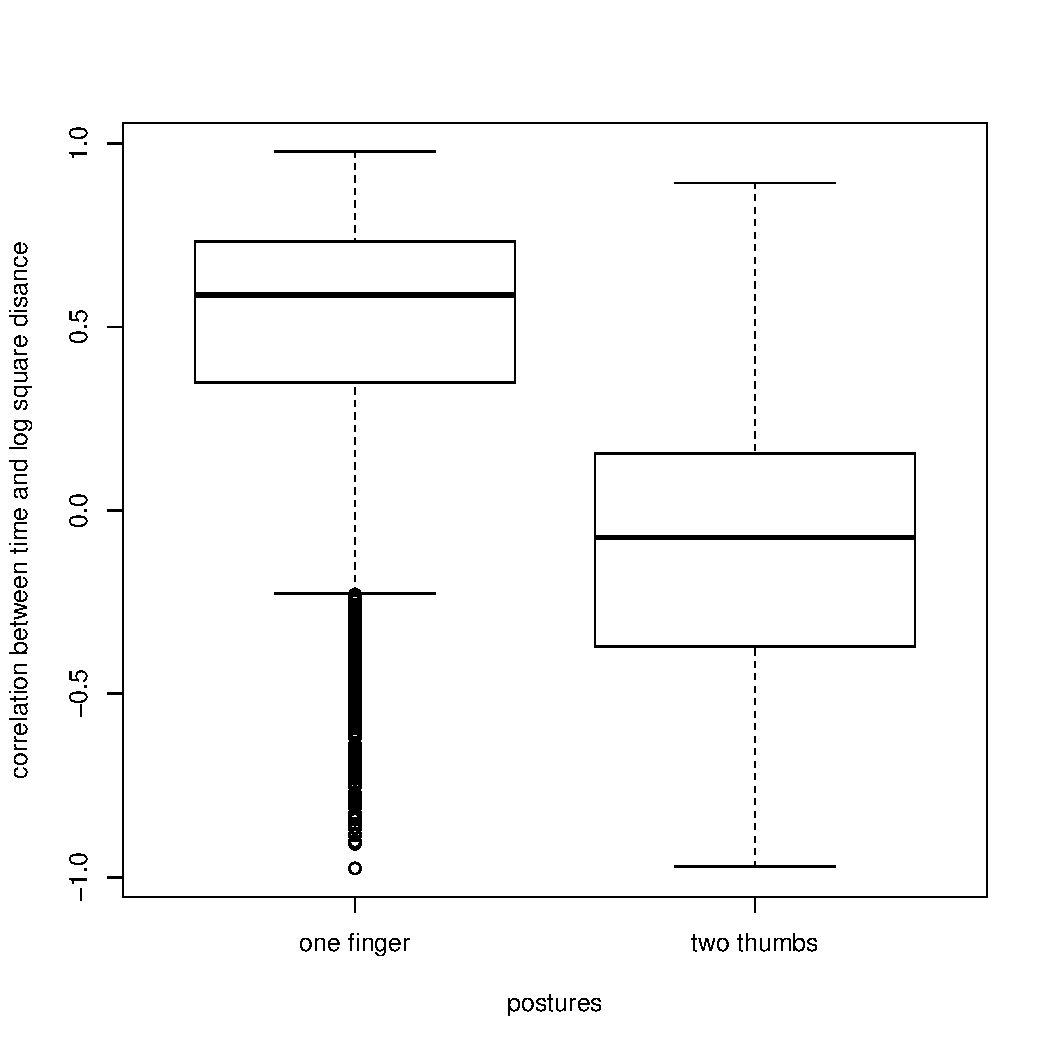
\includegraphics[width=1\columnwidth]{figures/boxplot.pdf}
  \caption{Correlation between time elapsed and log square distance between
  consecutive key presses for every 10 keys. There is a stronger correlation for
  one- finger input than that for two-thumb input.}
  \label{fig:boxplot}
\end{figure}

3. User adaptation

Fig. 5  A look at how key detection accuracy changes as the number of tapping points used for building the user adaptive Gaussian model for key ‘E’ increases
4. Key detection process 

\section{Implementation and simulation}
In the decoding process, a higher order more specialized model is used if it
meets a set of conditions such as a particular posture mode is detected with high confidence and the corresponding model (e.g. h/t, one-finger) is available (live, matured). Otherwise we back off to a lower order model, all the way to a base model which is key, individual and posture independent if necessary.

We did simulation using 20 users' data for training both the posture
classifier and spatial model, and tested on the other 10 users' data. The
percentages of one finger input and two thumbs input postures are the same in
both the training and testing data sets.

\begin{table}[tb]
  \centering
  \begin{tabularx}{\columnwidth}{|X|c|}
  \hline
  \tabhead{Spatial model} & \tabhead{Error rate} \\
  \hline
  Spherical cov & 8.693\% \\
  \hline
  Learned covariance & 91.359 \\
  \hline
  Key adaptive  & 91.292 \\
  \hline
  Posture and key adaptive  & 91.598 \\
  \hline
  User and key adaptive & 91.7438 \\
  \hline
  User and key adaptive (combine user and population Gaussian)  & 91.486\% \\
  \hline
  User and key adaptive (combine user and population, distance only) &  92.700\%
  \\
  \hline
  \end{tabularx}
  \caption{Off device simulation result}
  \label{tab:off-device}
\end{table}

\begin{figure}[tb]
  \centering
  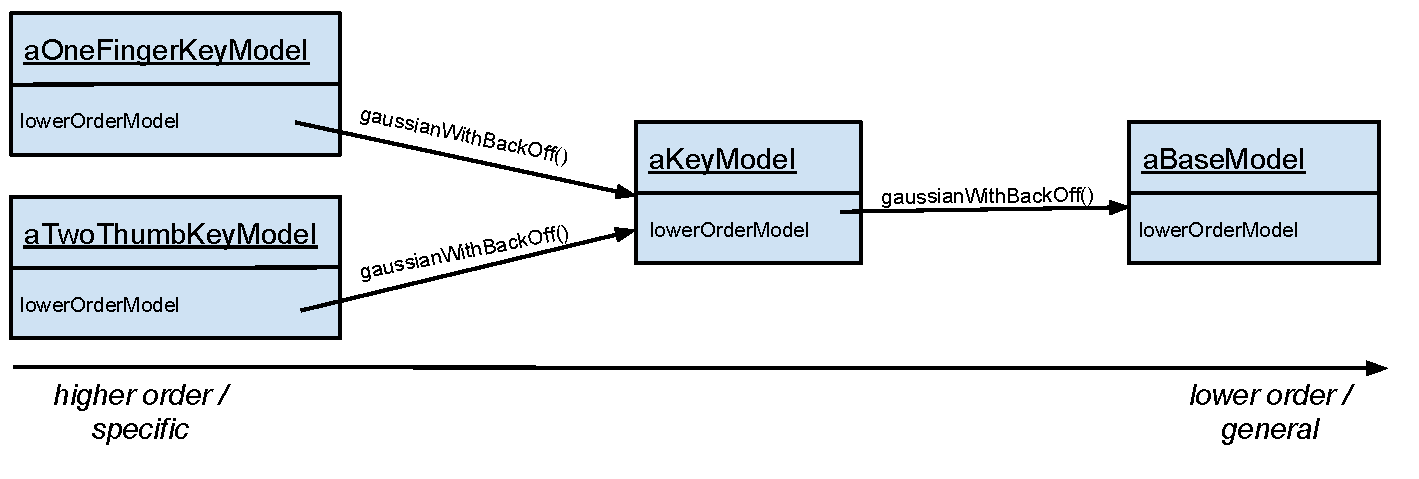
\includegraphics[width=1\columnwidth]{figures/chain-of-responsibility.pdf}
  \caption{Tapping points data from input on a Nexus S phone.}
  \label{fig:time-distance}
\end{figure}

\begin{figure}[tb]
 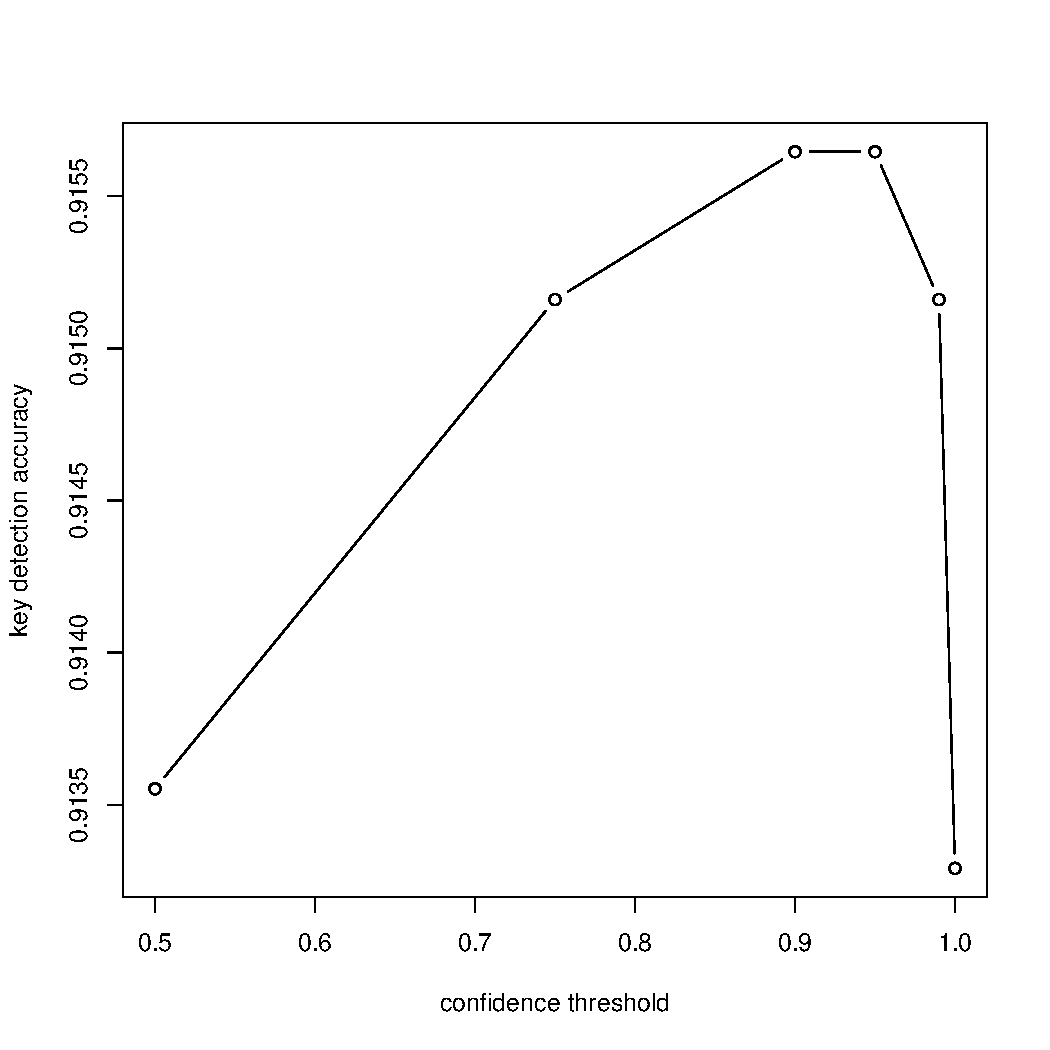
\includegraphics[width=1\columnwidth]{figures/posture-confidence.pdf}
  \caption{Tapping points data from input on a Nexus S phone.}
  \label{fig:time-distance}
\end{figure}

\begin{figure}[tb]
 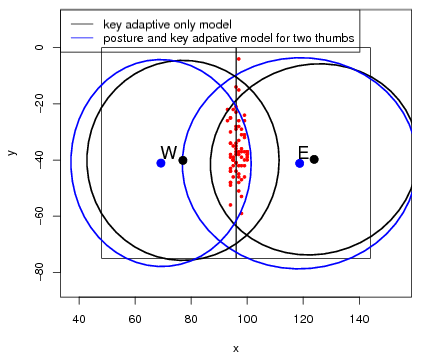
\includegraphics[width=1\columnwidth]{figures/key-posture-ellipse.png}
  \caption{Comparison of Gaussian distributions.}
  \label{fig:time-distance}
\end{figure}

\begin{figure*}[tb]
	\centering
	\subfigure[Key adaptive model]{
    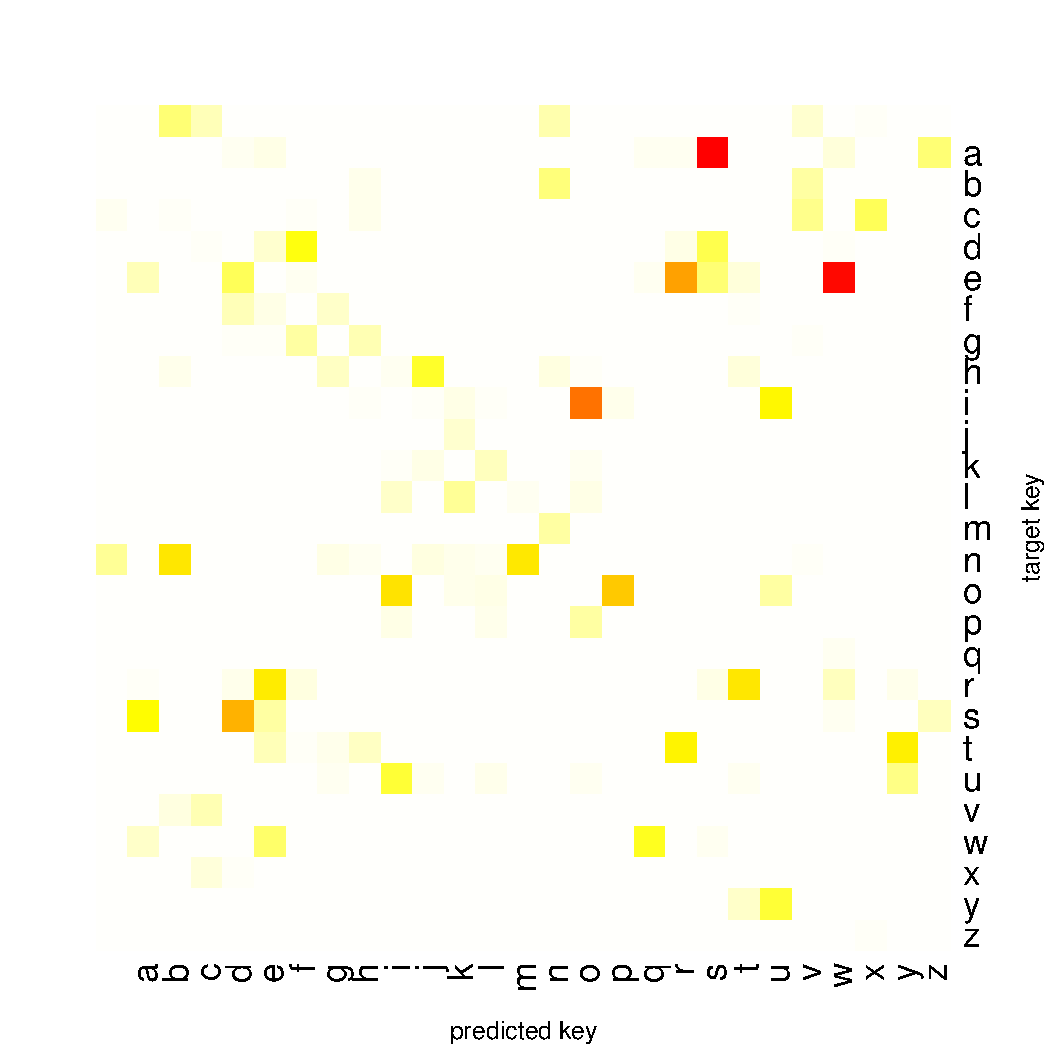
\includegraphics[width=0.49\columnwidth]{figures/sim-result-1.pdf}
    \label{fig:subfig1}
	} 
	\subfigure[Caption of subfigure 2]{
    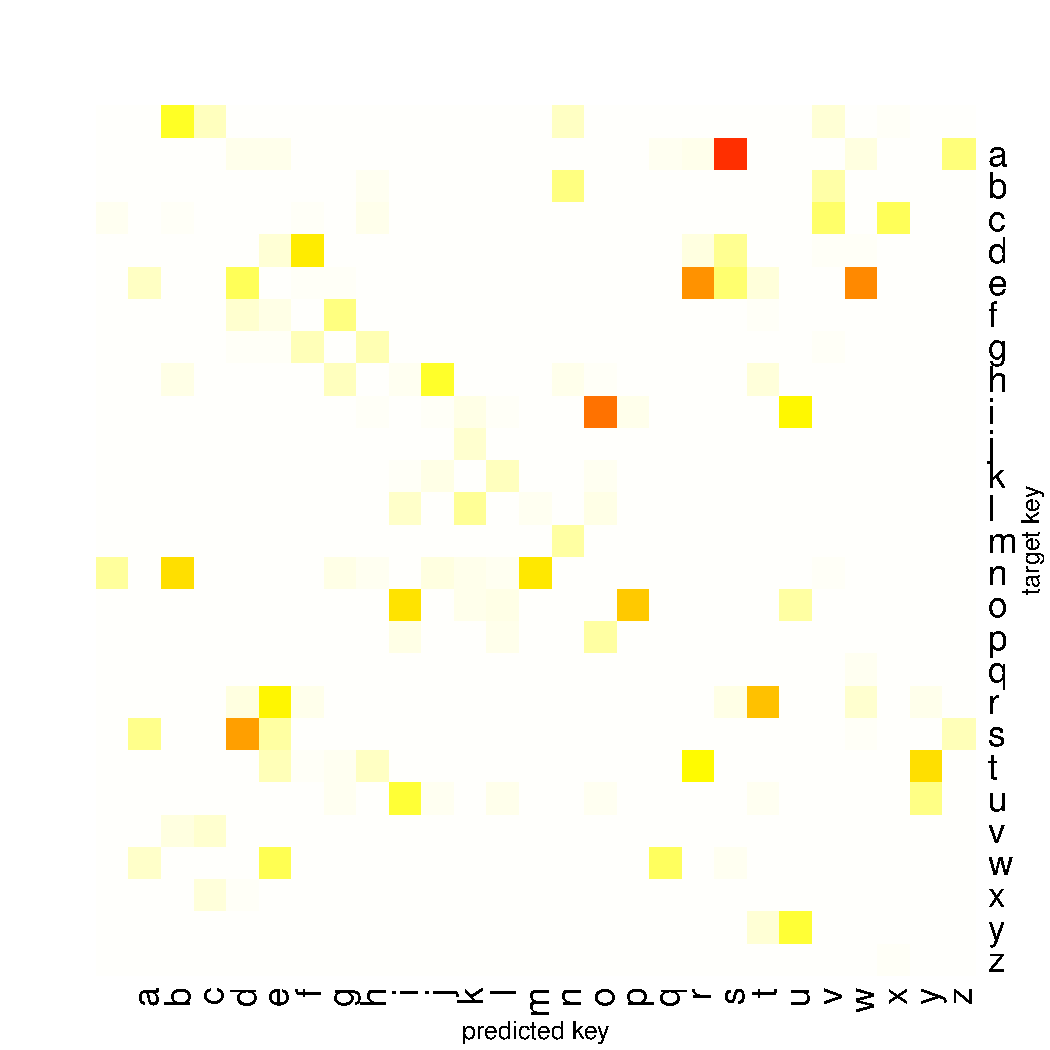
\includegraphics[width=0.49\columnwidth]{figures/sim-result-2.pdf}
    \label{fig:subfig2}
	}
	\subfigure[Caption of subfigure 3]{
    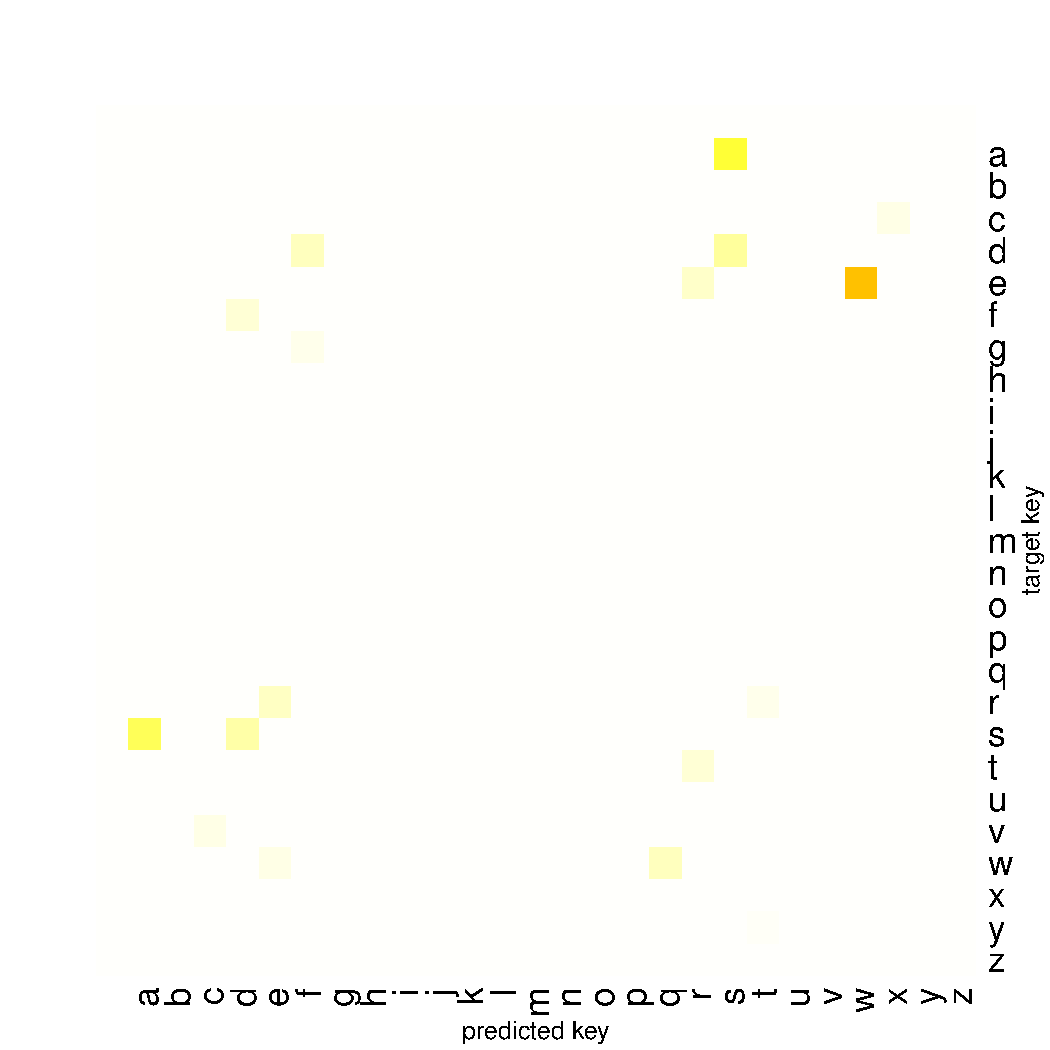
\includegraphics[width=0.49\columnwidth]{figures/sim-result-1-2.pdf}
    \label{fig:subfig3}
	}
	\subfigure[Caption of subfigure 3]{
    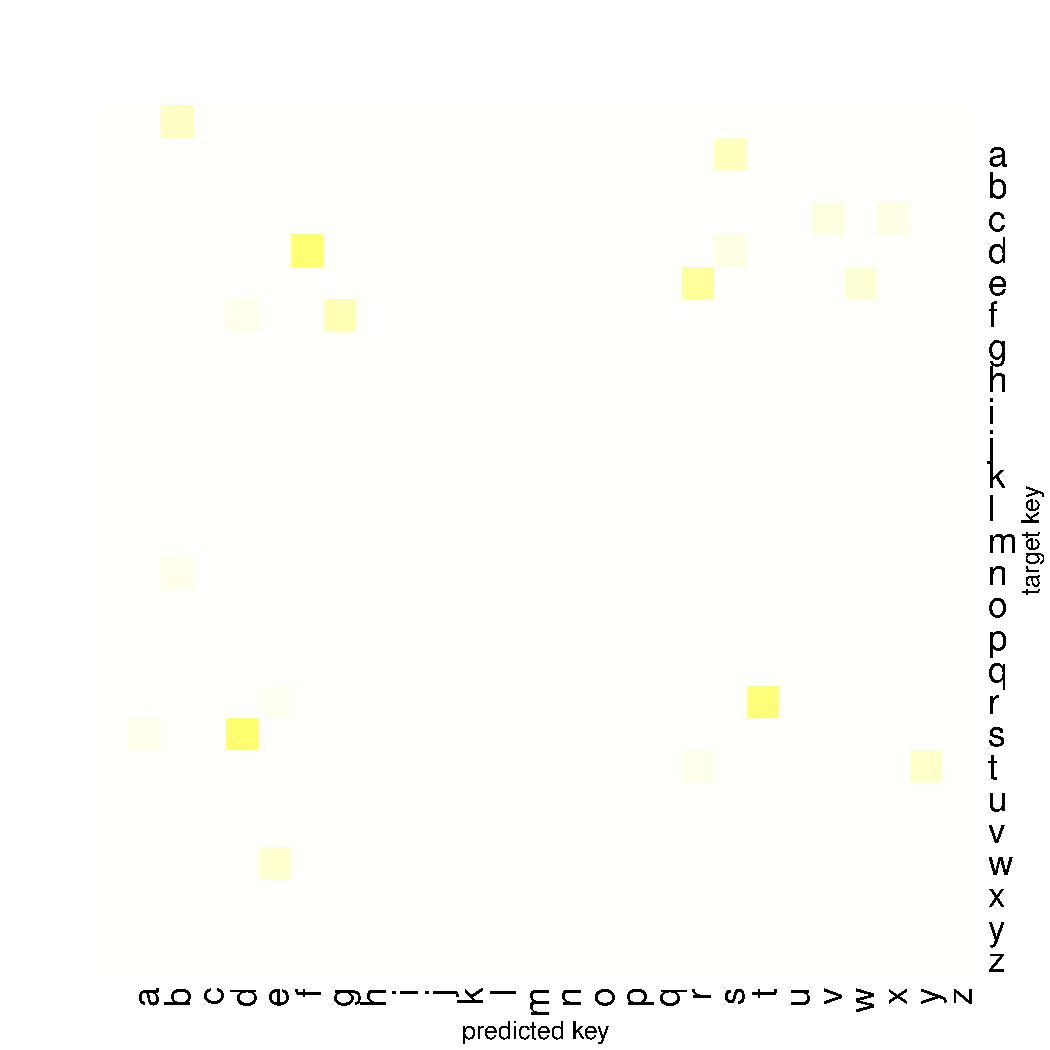
\includegraphics[width=0.49\columnwidth]{figures/sim-result-2-1.pdf}
    \label{fig:subfig3}
	}
	\caption[Optional caption for list of figures]{Caption of subfigures
	\subref{fig:subfig1}, \subref{fig:subfig2} and \subref{fig:subfig3}}
	\label{fig:subfigureExample}
\end{figure*}

\section{On-device simulation with language model}

\section{Conclusion}

It is important that you write for the SIGCHI audience.  Please read
previous years' Proceedings to understand the writing style and
conventions that successful authors have used.  It is particularly
important that you state clearly what you have done, not merely what
you plan to do, and explain how your work is different from previously
published work, i.e., what is the unique contribution that your work
makes to the field?  Please consider what the reader will learn from
your submission, and how they will find your work useful.  If you
write with these questions in mind, your work is more likely to be
successful, both in being accepted into the Conference, and in
influencing the work of our field.

\section{Acknowledgments}

We thank all the volunteers, and all publications support
and staff, who wrote and provided helpful comments on previous
versions of this document.  Some of the references cited in this paper
are included for illustrative purposes only.  \textbf{Don't forget
to acknowledge funding sources as well}, so you don't wind up
having to correct it later.

% Balancing columns in a ref list is a bit of a pain because you
% either use a hack like flushend or balance, or manually insert
% a column break.  http://www.tex.ac.uk/cgi-bin/texfaq2html?label=balance
% multicols doesn't work because we're already in two-column mode,
% and flushend isn't awesome, so I choose balance.  See this
% for more info: http://cs.brown.edu/system/software/latex/doc/balance.pdf
%
% Note that in a perfect world balance wants to be in the first
% column of the last page.
%
% If balance doesn't work for you, you can remove that and
% hard-code a column break into the bbl file right before you
% submit:
%
% http://stackoverflow.com/questions/2149854/how-to-manually-equalize-columns-
% in-an-ieee-paper-if-using-bibtex
%
% Or, just remove \balance and give up on balancing the last page.
%
\balance

% If you want to use smaller typesetting for the reference list,
% uncomment the following line:
% \small
\bibliographystyle{acm-sigchi}
\bibliography{chi2013}
\end{document}
